\section{Systemmodelle}

\subsection{Globale Testfälle}
Folgende Funktionssequenzen sind zu überprüfen:

\begin{itemize}
\item \textbackslash T10 \textbackslash Funktionssequenzbeschreibung
\end{itemize}

\subsection{Datenkonsistenzen}

\begin{itemize}
\item \textbackslash T30 \textbackslash Datenkonsistenzbeschreibung
\end{itemize}

\subsection{Objektmodell}
% UML Klassendiagramme

\begin{figure}[h]
\centering
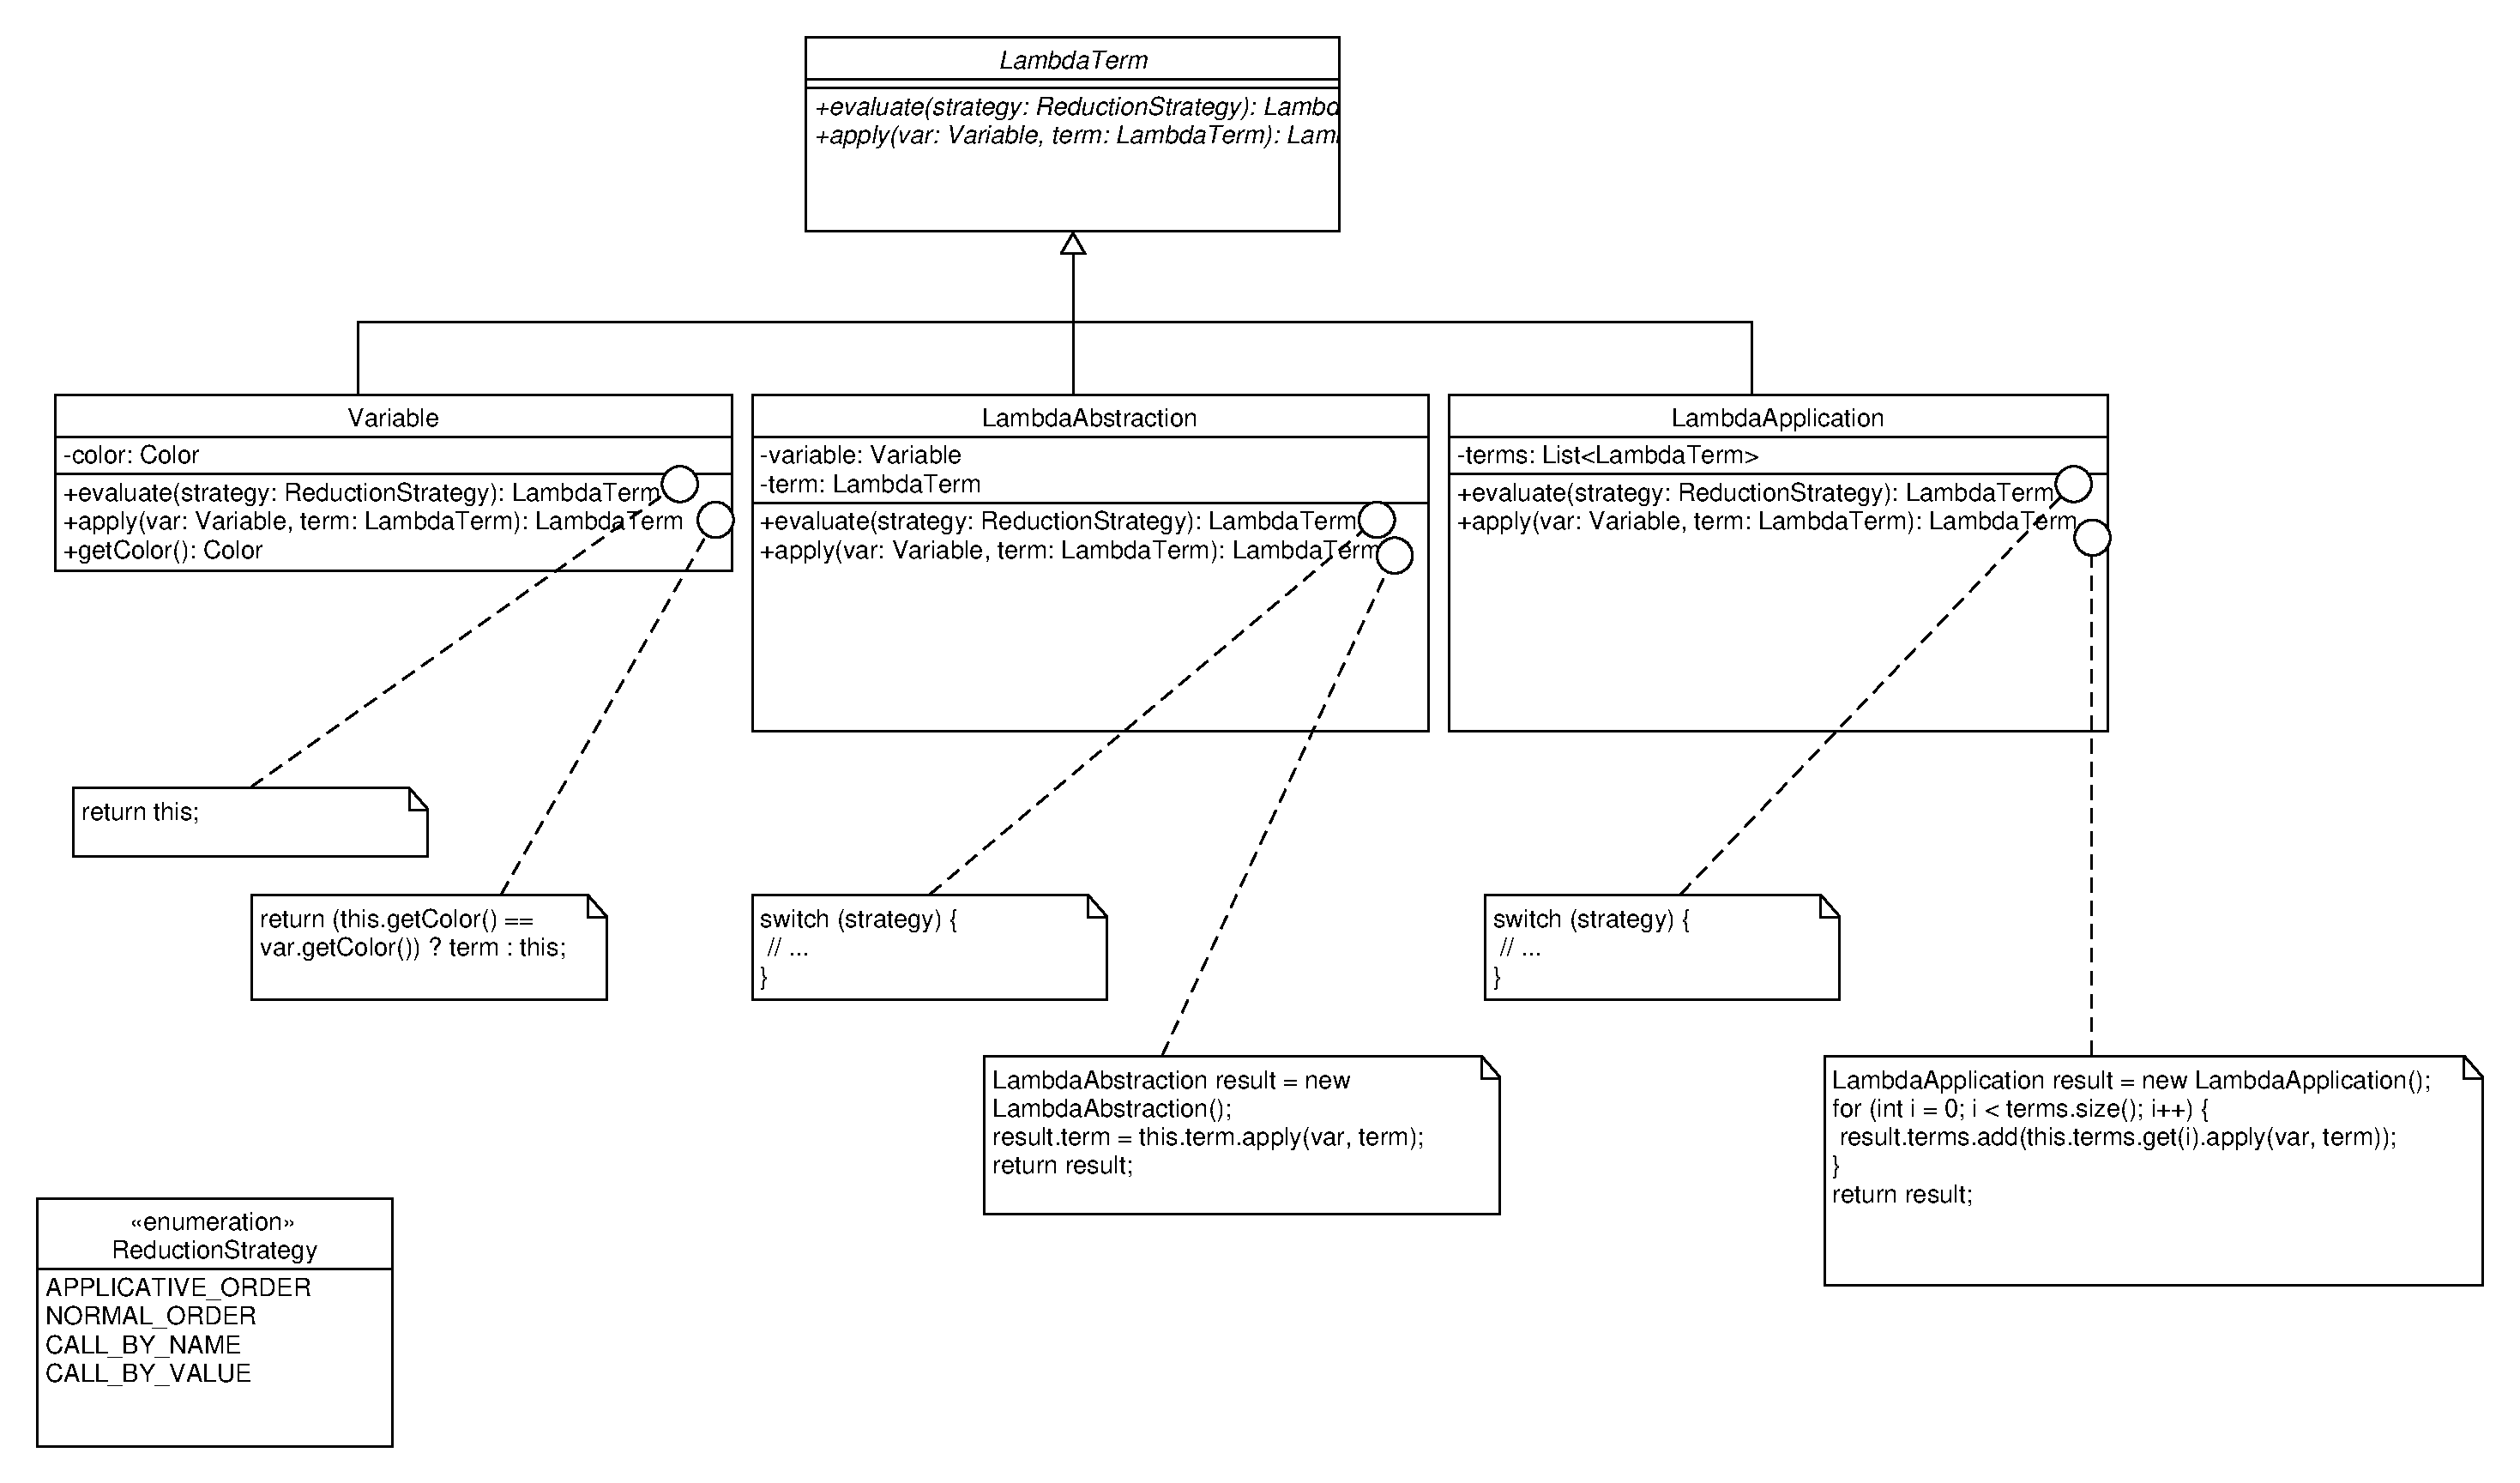
\includegraphics[scale=0.35]{../system_models/object_models/lambda_calculus.pdf}
\caption{UML Klassendiagramm zum Lambda-Kalkül}
\end{figure}

\subsection{Dynamische Modelle}
% UML Zustandsautomat, Sequenzdiagramm

\begin{figure}[h]
\centering
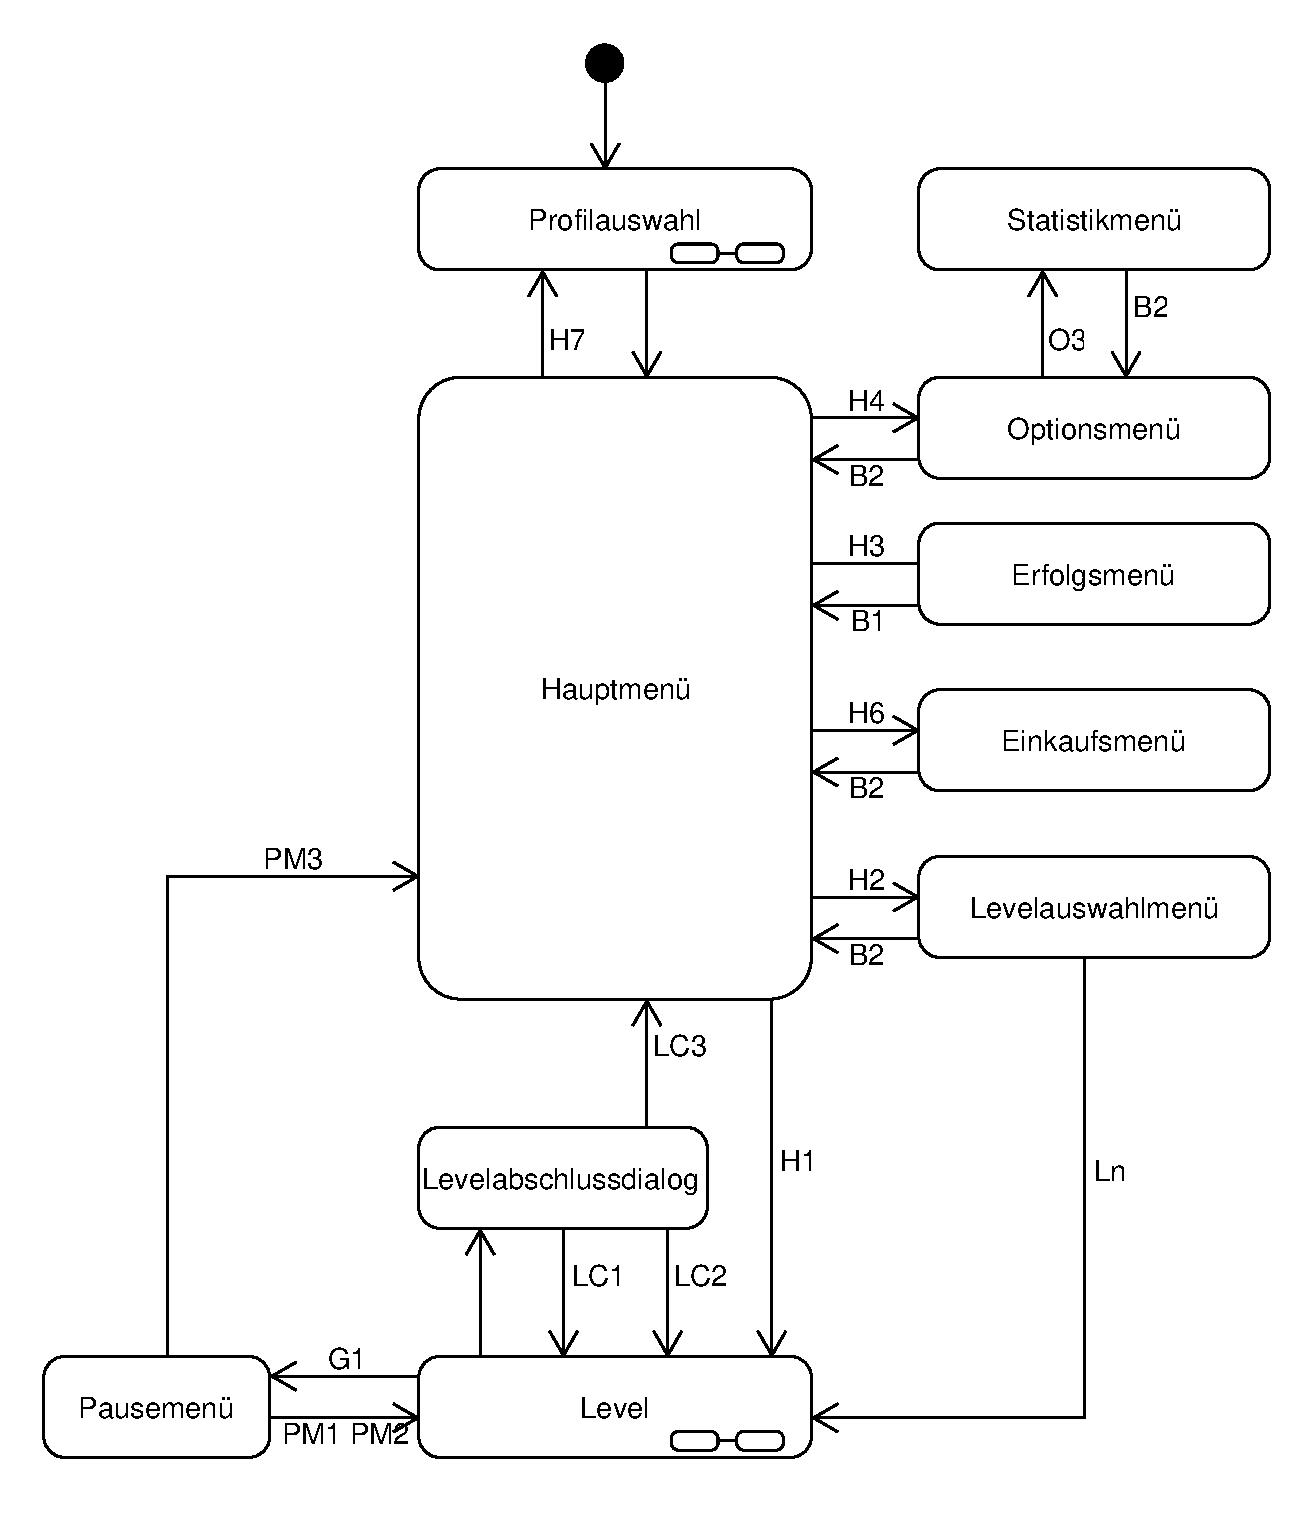
\includegraphics[scale=0.3]{../system_models/dynamic_models/menu_state_machine.pdf}
\caption{Zustandsautomat zur Menübedienung}
\end{figure}

\begin{figure}[h]
\centering
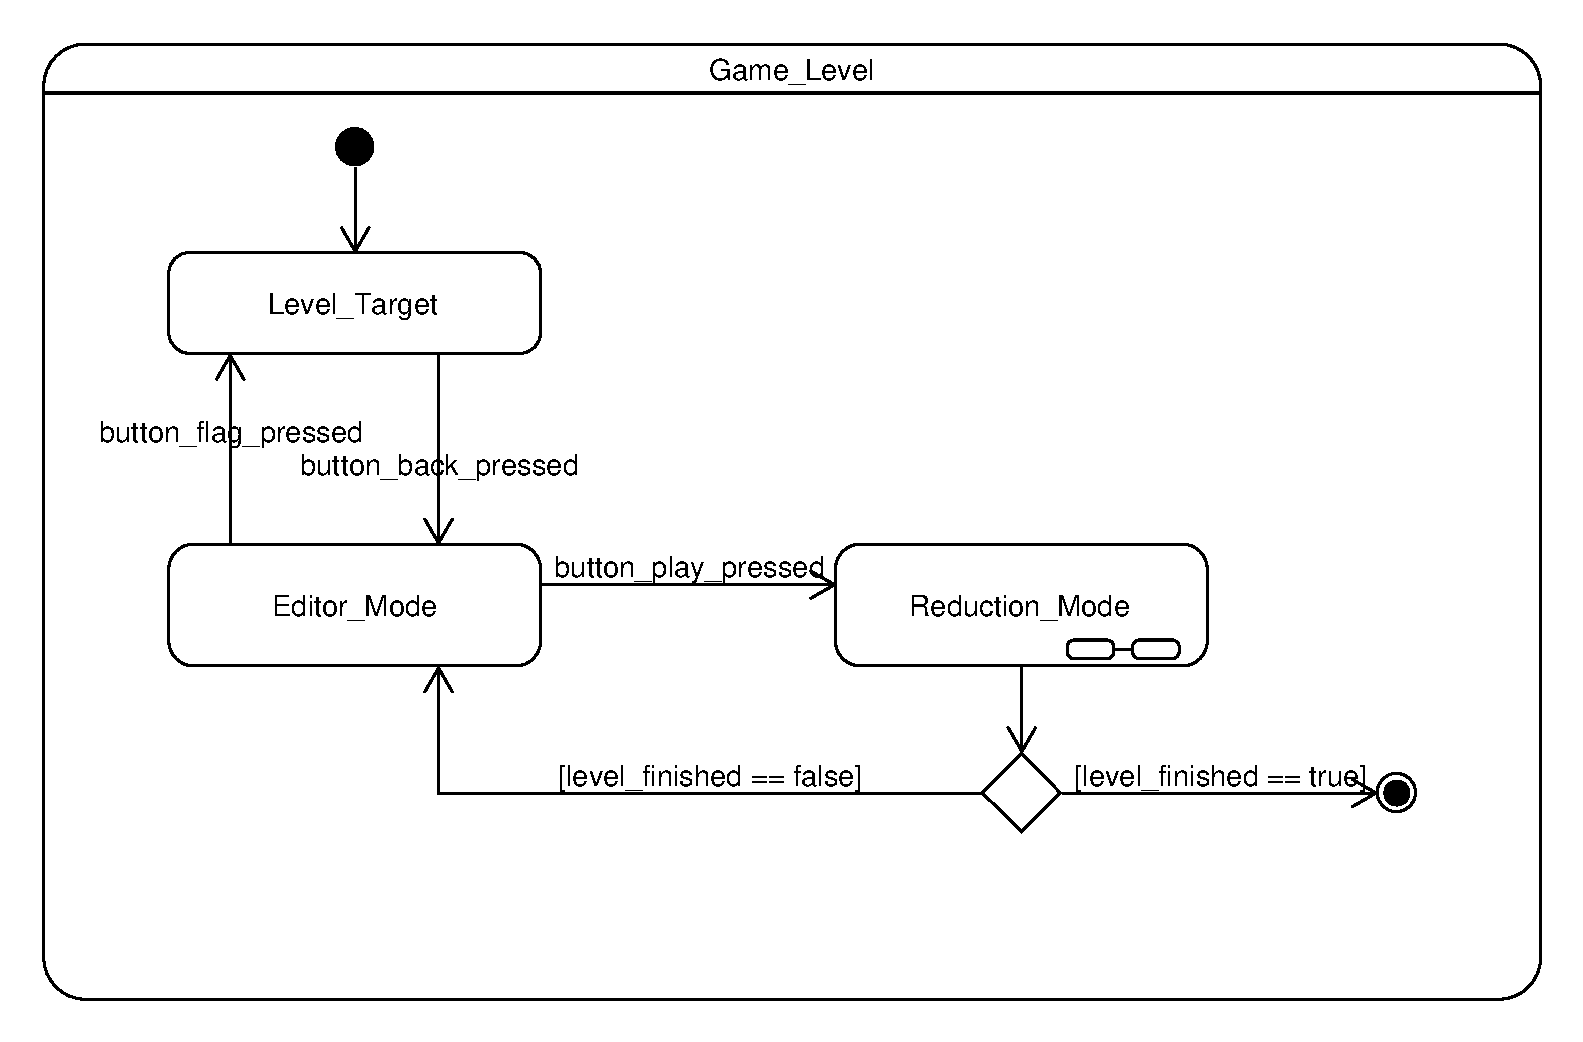
\includegraphics[scale=0.6]{../system_models/dynamic_models/game_level_state_machine.pdf}
\caption{Zustandsautomat zum Ablauf eines Levels}
\end{figure}

\begin{figure}[h]
\centering
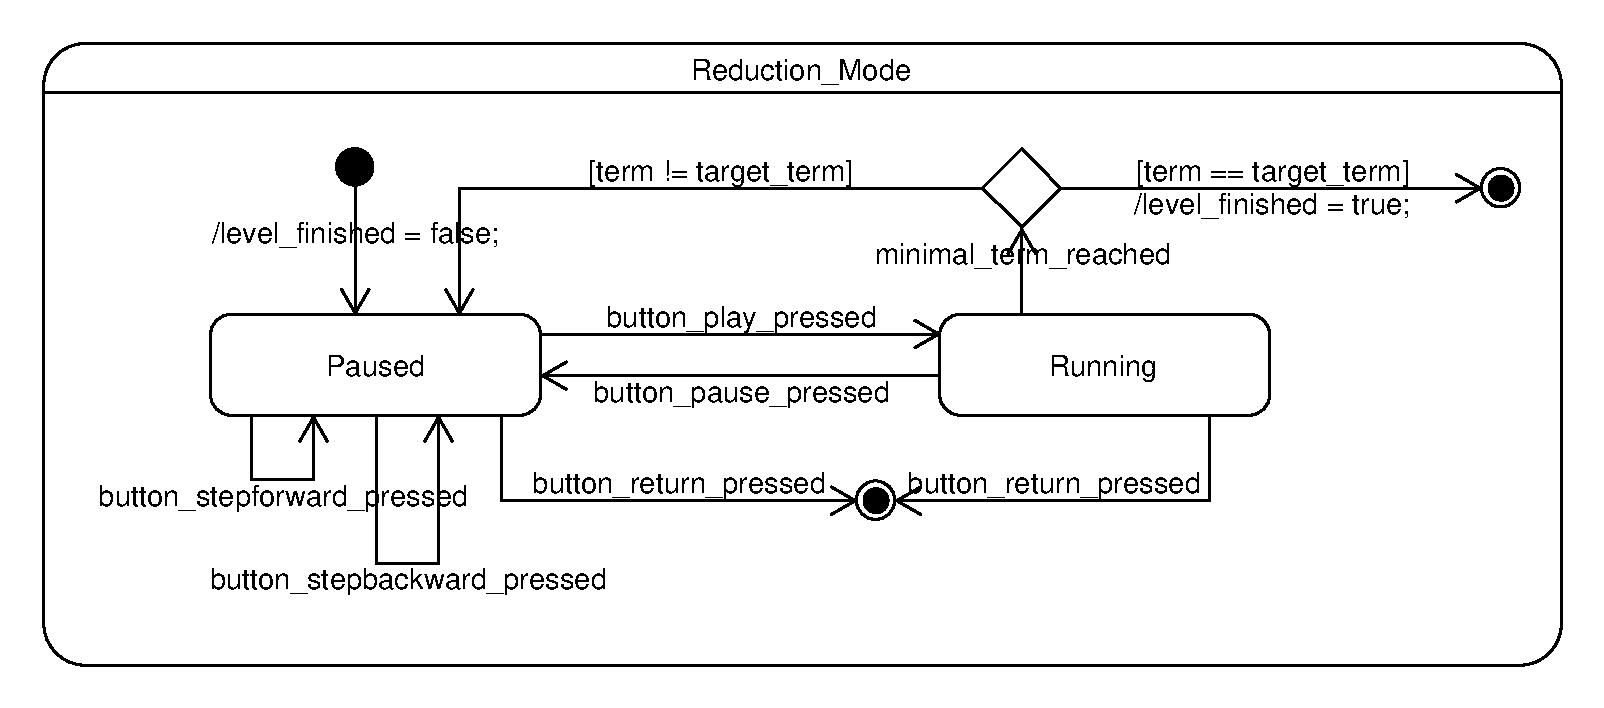
\includegraphics[scale=0.6]{../system_models/dynamic_models/reduction_mode_state_machine.pdf}
\caption{Zustandsautomat zur Funktion des Reduktions-Modus}
\end{figure}

\subsection{Benutzerschnittstelle}

GUI